\documentclass[11pt]{article}

\usepackage[utf8]{inputenc}
\usepackage[T1]{fontenc}
\usepackage{amsmath}
\usepackage{amssymb}
\usepackage{mathtools}
\usepackage{graphicx}
\usepackage{float}
\usepackage[left=10mm,right=10mm]{geometry}
\usepackage{booktabs}
\usepackage{array}
\usepackage{enumitem}
\usepackage{fancyhdr}
\usepackage{subfig}
\usepackage{multirow}
\usepackage[ruled, lined, vlined, linesnumbered, commentsnumbered, longend]{algorithm2e}
\usepackage[activate={true,nocompatibility},final,tracking=true,kerning=true,spacing=true,factor=1100,stretch=10,shrink=10]{microtype}
\usepackage[margin=10pt,font=small,labelfont=bf,labelsep=endash]{caption}

% Refererencing
\usepackage[backend=biber,style=alphabetic]{biblatex}

\microtypecontext{spacing=nonfrench}

\graphicspath{ {./images/} }

\newcommand{\derivative}[2]{\frac{\partial #1}{\partial #2}}
\newcommand{\suml}[2]{\sum\limits_{#1}^{#2}}

\pagestyle{fancy}
\fancyhf{}
\setlength{\headheight}{14pt}
\rhead{\thepage}
\lhead{Assignment 5}

\begin{document}

\date{\today}
\author{Sanchit Nevgi}

\section{Derivation of likelihood}

We are given $p(y | x, z) = \sigma(y z^T x)$, where $\sigma(x) = 1 / (1 + \exp(-x))$.

\begin{equation}
    \begin{aligned}
        \log p(y | x, z) & = \log \frac{1}{1 + \exp(-y z^T x)}                                              \\
                         & = \log 1 - \log (1 + \exp(-y z^T x))                                             \\
                         & = 0 - \log (\exp(0) + \exp(-y z^T x))                                            \\
                         & = - lae(0, -y z^T x) \;\; \text{,where} \;\; lae(s, t) = \log(\exp(s) + \exp(t))
    \end{aligned}
\end{equation}

\section{Derivation of gradient}

\begin{equation}
    \begin{aligned}
        \derivative{}{t} lae(s, t) & = \derivative{}{t} \log(\exp(s) + \exp(t))                         \\
                                   & = \frac{1}{\exp(s) + \exp(t)} \derivative{}{t} (\exp(s) + \exp(t)) \\
                                   & = \frac{\exp(t)}{\exp(s) + \exp(t)}                                \\
                                   & = \frac{1}{1 + \exp(s - t)} = \sigma(t - s)
    \end{aligned}
\end{equation}

\begin{equation}
    \begin{aligned}
        \nabla_z \log p (y|x,z) & = \nabla_z -lae(0, -yz^Tx)                  \\
                                & = - \nabla_z lae(0, -yz^Tx)                 \\
                                & = - \sigma(-yz^Tx - 0) \nabla_z (- y z^T x) \\
                                & = - \sigma(-yz^Tx) -yx                      \\
                                & = \sigma(-yz^Tx) yx
    \end{aligned}
\end{equation}

\clearpage
\section{Pseudocode for Stochastic gradient variational inference}

We use $\mathcal{N} (w, 0.5 I)$ as our variational distribution $q_w (z)$. We can approximately compute $\int q_w (z) \log p(z, Data) \mathrm{d}z$ by taking samples from $q_w (z)$ and computing $\log p (z, Data)$. Since $x$ is observed, we avoid modeling it. Further we assume the prior to be a standard unit normal.

\begin{algorithm}[!htbp]
    \SetAlgoLined
    \KwIn{w}
        $z \backsim q_w(z) \backsim \mathcal{N}(w, 0.5 I)$ \;
        Compute $\log p(z, Data)$ as \;
        $ = \log \left( p(z) \prod\limits_{i = 1}^N \log p(y^{(i)}|x^{(i)}, z) \right) = \log \exp (\frac{-1}{2} \Vert z \Vert^2) + \suml{i=1}{N} \log p(y^{(i)}|x^{(i)}, z)$ \;
        $evidence = \frac{-1}{2} \Vert z \Vert^2 + \suml{i=1}{N} lae(0, -y z^T x^{(i)})$ \;
    \Return evidence 
     \caption{Estimating Mean Evidence}
\end{algorithm}

\begin{algorithm}[!htbp]
    \SetAlgoLined
    \KwIn{w}
        $z \backsim \mathcal{N}(w, 0.5 I)$ \;
        \tcc{Using reparameterization trick, ignoring entropy due to fixed covariance}
        $\nabla_w \mathbb{ELBO}  = \nabla_w \frac{-1}{2} \Vert T_w(\epsilon) \Vert^2 + \nabla_w \suml{i=1}{N} lae(0, -y T_w(\epsilon)^T x^{(i)})$ \;
        \tcc{Using $T_w(\epsilon) = z$}
        $\nabla_w \mathbb{ELBO} = -z + \suml{i = 1}{N} \sigma(-y^{(i)} z^T x^{(i)}) y^{(i)} x^{(i)} $ \;
        \Return $\nabla_w \mathbb{ELBO}$
     \caption{Gradient of Mean Evidence}
\end{algorithm}

\section{Implement SGVI}

\begin{figure}[H]
    \centering
    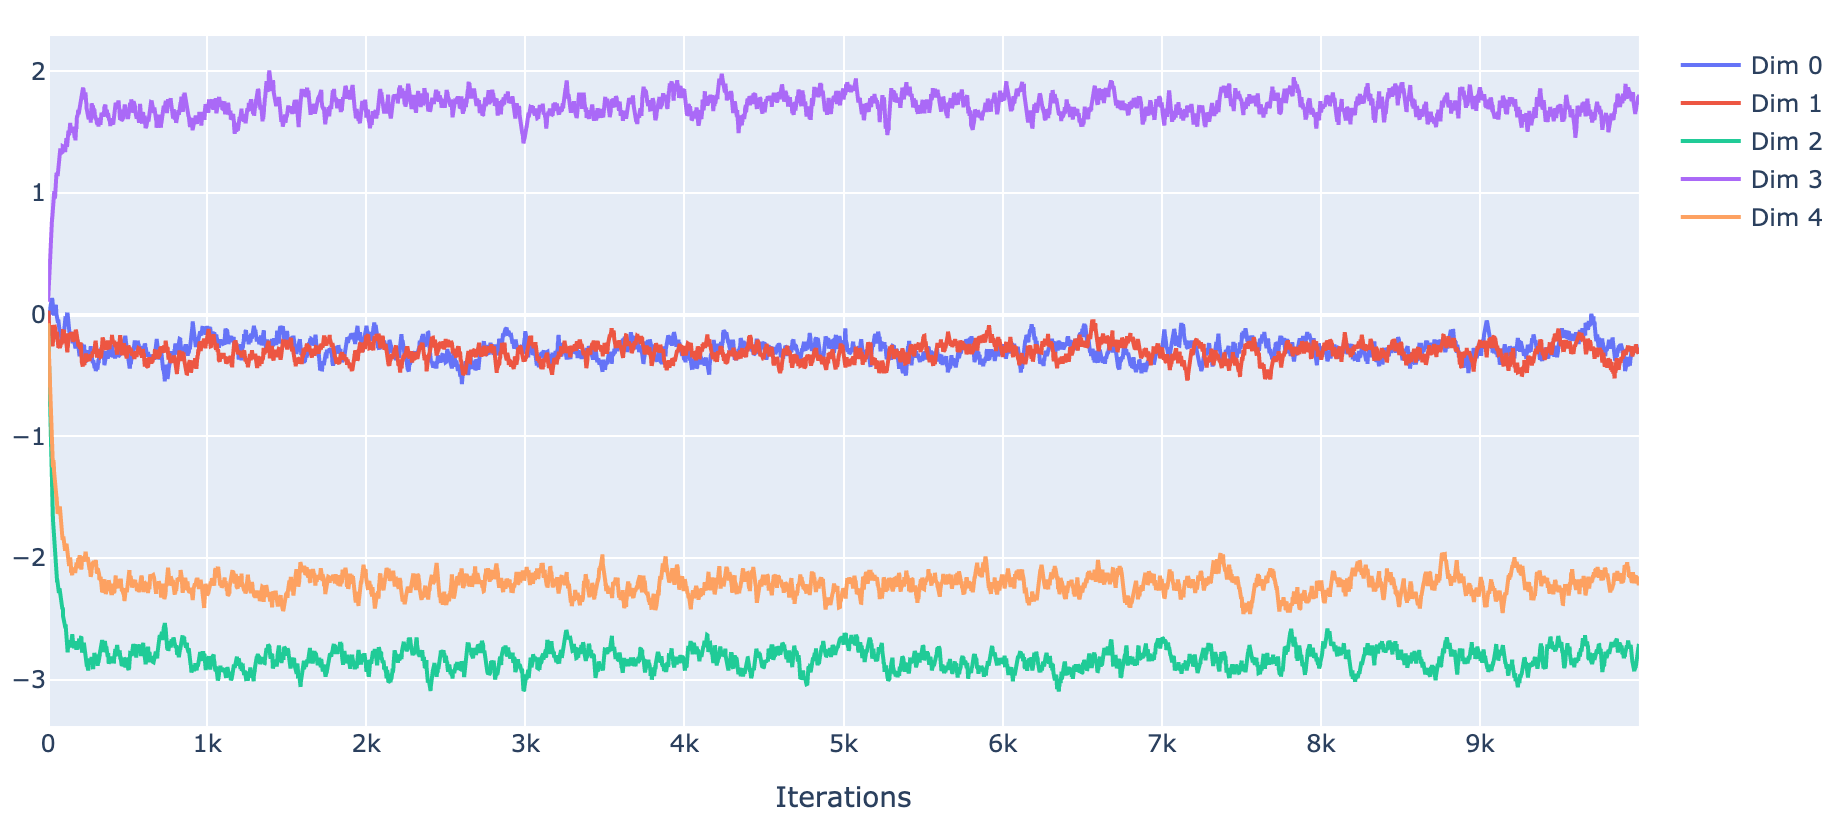
\includegraphics[width=\textwidth]{./images/w-plot.png}
\end{figure}

\clearpage
\section{Direct predictive accuracy for SGVI}

\subsection{Prediction using samples}

For a new test input $x$, we sample $z_1, z_2, ... z_{t_{max}}$ from the posterior $p(z|Data)$. We compute the mean of each prediction, which is the sigmoid of the dot product of the sample and test input.

\begin{equation}
    p(y = 1) =  \frac{1}{t_{max}} \suml{i = 1}{t_{max}} \sigma (x^T z_i )
\end{equation}

\subsection{Error rates}

\begin{table}[!htbp]
    \centering
    \begin{tabular}{cl|ccccc}
        \toprule
        & & \multicolumn{5}{c}{Repetitions} \\
        \midrule
        \multirow{4}{*}{\rotatebox{90}{Iterations}} & 10 & 0.149 & 0.205 & 0.155 & 0.153 & 0.159 \\
        & 100 & 0.147 & 0.144 & 0.146 & 0.15  & 0.144 \\
        & 1000 & 0.143 & 0.147 & 0.145 & 0.139 & 0.14  \\
        & 10000 & 0.145 & 0.144 & 0.145 & 0.144 & 0.143 \\
        \bottomrule
    \end{tabular}
    \caption{Error rates for increasing iterations across 5 repetitions}
\end{table}

\clearpage
\section{Step Sizes and Run Lengths for SGVI Dynamics}

We experiment with different step sizes and iterations. To measure performance, we evaluate on the test set at specified intervals. We plot the error rates subsequently.

\begin{figure}[!htbp]
    \centering
    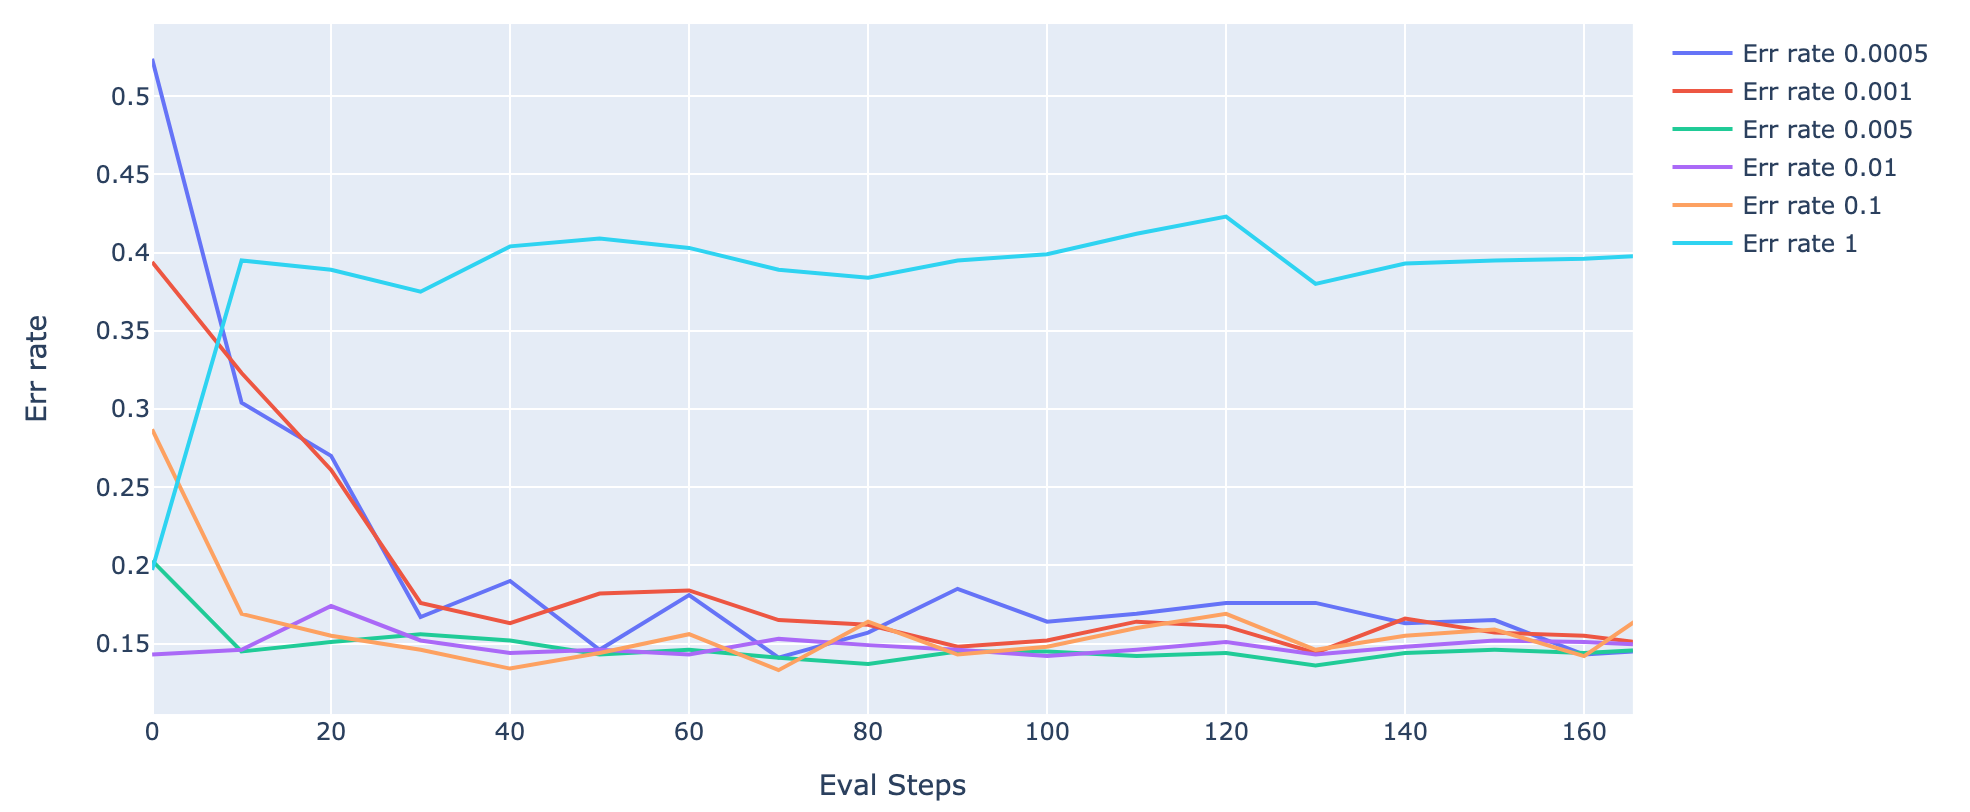
\includegraphics[width=\textwidth]{./images/step-sizes.png}
    \caption{Average performance as measured by error rate for different step sizes. Number of iterations fixed to 1000, evaluated every 20 steps}
\end{figure}

\begin{figure}[!htbp]
    \centering
    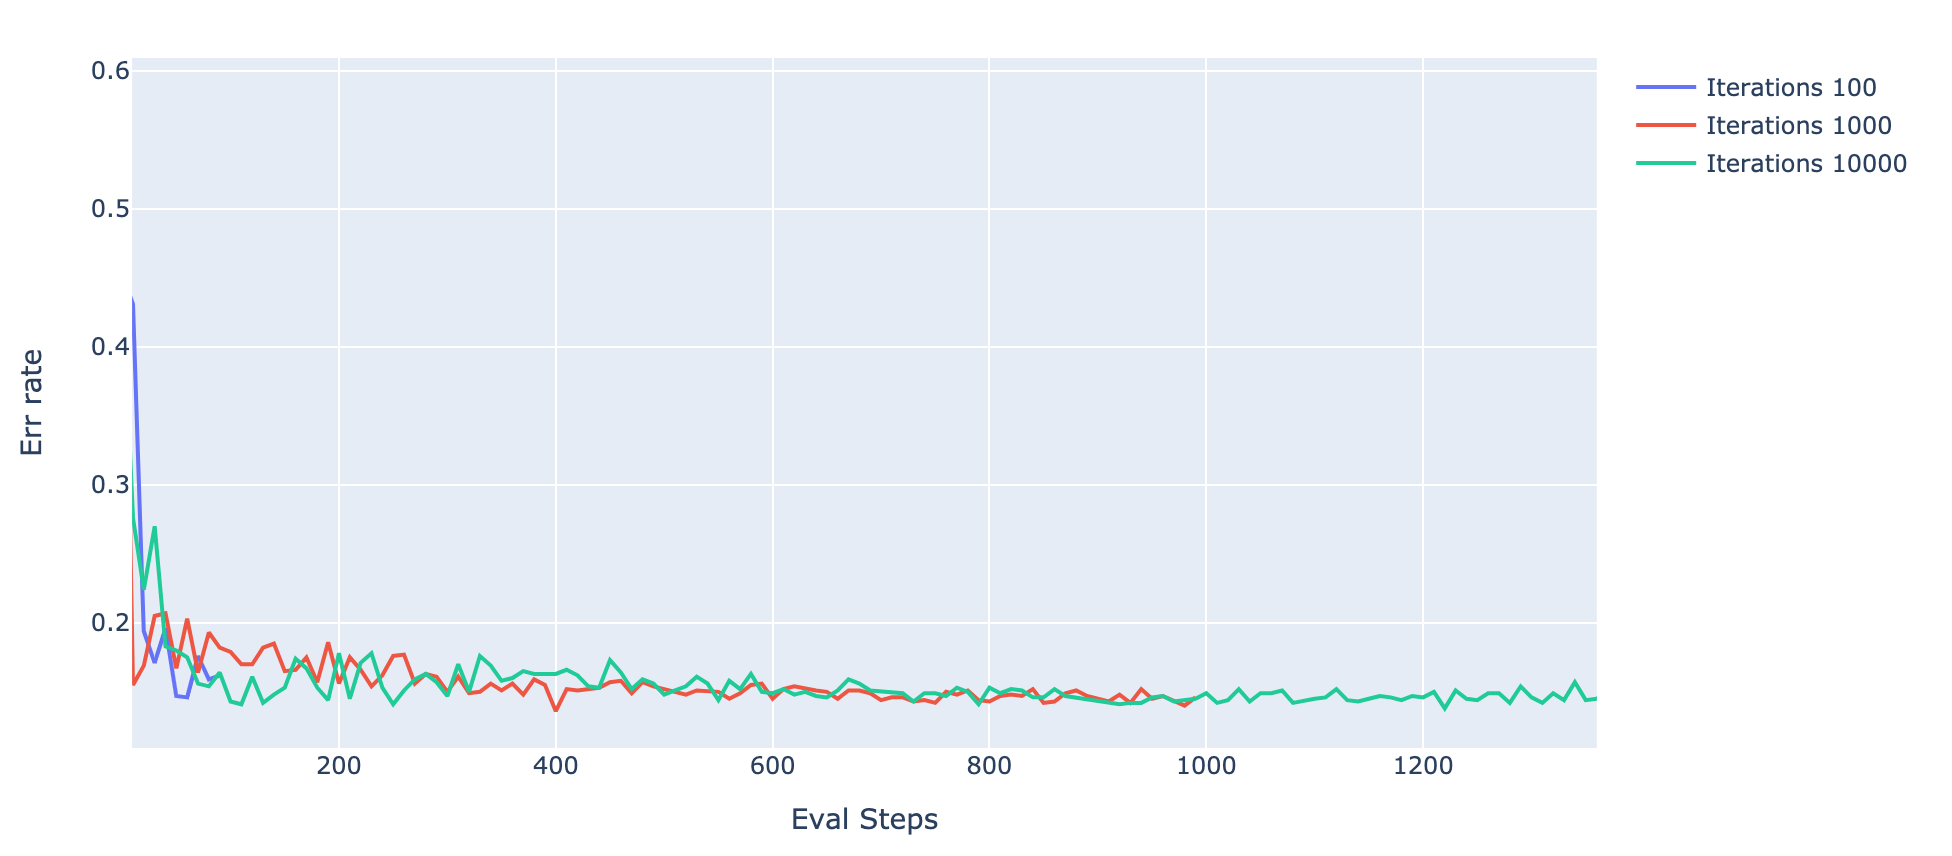
\includegraphics[width=\textwidth]{./images/iterations.png}
    \caption{Checking convergence acorss different run lenghts}
\end{figure}

We see that the error rates converges after approximately 1000 iterations. As expected a larger step size, leads to faster convergence. However, setting a very large step-size $= 1$, causes divergence, as seen from the figure.

\end{document}